\chapter{Abordagens Evolucionárias para a TMAP}
\label{chp:abordagens}

No último capítulo, foram apresentados os algoritmos evolucionários usados nesta 
pesquisa. No entanto, algumas lacunas ficaram abertas: não foram apresentadas 
formas de gerar indivíduos, isto é, soluções para a \ac{tmap}, de forma 
arbitrária para a primeira população, além de como aplicar 
recombinação e mutação neles. A definição desses operadores depende da forma 
escolhida para representar indivíduos. Tipicamente, na literatura de Algoritmos 
Evolucionários, indivíduos são representados como um vetor de bits ou de números 
reais \citep{Luke2013Metaheuristics}. No entanto, tal como foi apresentado na 
\secref{definicoes_tmap}, a \ac{tmap} não é representada naturalmente por essas 
estruturas de dados.

Considerando estas questões de representação, esta pesquisa adota uma abordagem 
baseada em particionamento do grafo para resolver a \ac{tmap}, como foi sugerido 
por \citep{Chevaleyre:2004:TAM:1018411.1019013} e aplicado por 
\citep{Pippin:2013:PBT:2480362.2480378} e \citep{4630897}.

Cada agente pode ser representado por um ciclo que percorre todos os vértices de 
uma partição do grafo. Desta forma, uma solução para a \ac{tmap} seria 
representada (de forma finita) por um conjunto de $r$ ciclos que percorrem $r$ 
partições do grafo, onde $r$ é o número de agentes. Com isso, é possível trocar 
agentes entre soluções, que como será mostrado na \secref{sec:recombinacao}, é a 
base para a recombinação.

A partir deste modelo, foi adicionado o conceito de centro das partições para que 
a recombinação possa trocar agentes semelhantes. Se duas soluções possuem agentes 
com os mesmos centros de partição, será possível trocar os agentes que possuam o 
mesmo centro (o que não quer dizer partições iguais). O objetivo é fazer com que 
a troca envolva agentes que patrulhem regiões similares do grafo, mas caso não 
seja possível encontrar agentes com o mesmo centro nas duas soluções, a 
recombinação vai aplicar uma troca mais aleatória.

Finalmente, a representação proposta para uma solução da \ac{tmap} é: um conjunto 
de $r$ agentes, onde cada agente é representado por um ciclo que passa por todos 
os vértices de uma partição do grafo e um vértice de centro. A 
\figref{fig:tmap_example}, representa visualmente uma dessas soluções. Nela, 
dois agentes patrulham o grafo. Cada um ficou sob responsabilidade de uma 
partição, onde irão percorrer um ciclo indefinidamente. O agente vermelho, 
ficou com o centro $5$, enquanto que o verde com o centro 3.

\tikzstyle{vertex}=[circle,fill=black!25,minimum size=20pt,inner sep=0pt]
\tikzstyle{red vertex}=[circle,fill=red!25,minimum size=20pt,inner sep=0pt]
\tikzstyle{green vertex}=[circle,fill=green!25,minimum size=20pt,inner sep=0pt]
\tikzstyle{green edge} = [draw,line width=2pt,-,green!50]
\tikzstyle{red edge} = [draw,line width=2pt,-,red!50]

\begin{figure}
	\caption{Exemplo de solução da \ac{tmap}}
	\centering
	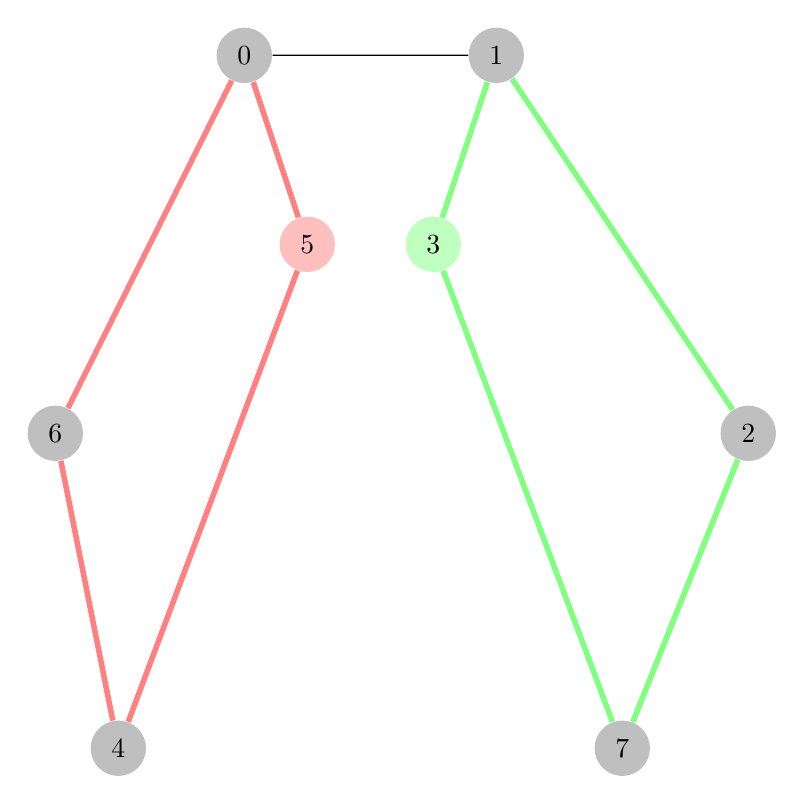
\begin{tikzpicture}
	[scale=.8,auto=left,every node/.style={circle,fill=blue!20}]
	\node[vertex] (n6) at (1,6)  {6};
	\node[vertex] (n0) at (4,12) {0};
	\node[vertex] (n1) at (8,12) {1};
	\node[vertex] (n2) at (12,6) {2};
	\node[vertex] (n4) at (2,1)  {4};
	\node[red vertex] (n5) at (5,9)  {5};
	\node[vertex] (n7) at (10,1) {7};
	\node[green vertex] (n3) at (7,9)  {3};
	
	\foreach \from/\to in {n0/n6,n6/n4,n4/n5,n5/n0}
		\path[red edge] (\from) -- (\to);
	\foreach \source/\dest in {n1/n2,n2/n7,n7/n3,n3/n1}
		\path[green edge] (\source) -- (\dest);
	\foreach \de/\para in {n0/n1}
		\draw (\de) -- (\para);
	
	\end{tikzpicture}
	\caption*{Fonte: O autor}
	\label{fig:tmap_example}
\end{figure}

Utilizando esta representação, serão propostos, neste capítulo, operadores 
para construção de indivíduos, mutação e recombinação.

\section{Criação de Indivíduos}

A criação de 
indivíduos foi dividida em três etapas. A primeira é o cálculo de $r$ centros, 
onde $r$ é o número de agentes. 
A segunda tarefa é a escolha dos vértices que compõem a partição, dentre os 
quais está o centro definido para ela. Por fim, falta o cálculo de um ciclo, 
para cada partição, que passe por todos os seus vértices. Essas tarefas foram 
chamadas respectivamente de \textit{centering}, \textit{partitioning} e 
\textit{path building}. No final, o resultado será um indivíduo (ou solução 
para a \ac{tmap}) com $r$ agentes, onde cada agente tem um vértice de centro e 
um caminho para percorrer durante a patrulha. Estes operadores são utilizados 
pelos algoritmos evolucionários no momento em que se precisa de um novo 
indivíduo gerado de forma aleatória (vide os pseudocódigos no 
\chapref{alg_evo}).

Nas subseções seguintes, cada uma dessas três tarefas será tratada 
separadamente, mas é importante notar que uma tarefa depende da resposta dada 
pela sua antecessora. Serão apresentados mais de um operador que executa cada 
tarefa, assim ao montar um algoritmo evolucionário, o leitor pode construir 
seus indivíduos com qualquer combinação deles.

\subsection{\textit{Centering}}

A primeira forma proposta para se calcular os centros é chamada de 
\textit{Random Centering}, e consiste em simplesmente escolher nós aleatórios do 
grafo para serem os centros. Veja o Pseudocódigo~\ref{centering_random} abaixo.

\begin{algorithm}                  % enter the algorithm environment
	\caption{\textit{Random Centering}}          % give the algorithm a caption
	\label{centering_random}                           % and a label for \ref{} commands later in the document
	\algcomment{\begin{center} Fonte: O Autor \end{center}}
	\begin{algorithmic}                    % enter the algorithmic environment
		\Procedure{RANDOM-CENTERING}{$V, r$}
		\newline
		\Comment{$V$ é o conjunto de vértices do grafo e $r$ é o número de agentes}
		\State $Vertices \gets $ Cópia($V$)
		\State $Centros \gets \{\}$
		\For{$1 ...\ r$}
			\State $Centros \gets Centros\ \cup$ \{Seleciona-Aleatoriamente-Remove($Vertices$)\}
		\EndFor
		\State \textbf{Retorne} $Centros$
		\EndProcedure
	\end{algorithmic}
\end{algorithm}

Uma outra forma de escolher os centros é tentar encontrar os vértices do grafo 
que estejam mais distantes uns dos outros. O objetivo neste operador é iniciar 
indivíduos de forma um pouco mais inteligente, para aumentar as chances de 
serem indivíduos com alta aptidão, mas sem perder completamente algum fator de 
aleatoriedade que é considerado importante nas inicializações de indivíduos nos 
algoritmos evolucionários. \citep{Luke2013Metaheuristics} alerta para os perigos 
de utilizar heurísticas que aparentam gerar melhores indivíduos, mas que podem 
estar, inadvertidamente, condenando os algoritmos evolucionários a ficarem 
"presos"\ em mínimos locais.

O pseudocódigo~\ref{centering_maximum} mostra como seria a implementação deste 
operador.

\begin{algorithm}                  % enter the algorithm environment
	\caption{\textit{Approximated Maximum Distance Centering}}          % give the algorithm a caption
	\label{centering_maximum}                           % and a label for \ref{} commands later in the document
	\algcomment{\begin{center} Fonte: O Autor \end{center}}
	\begin{algorithmic}                    % enter the algorithmic environment
		\Procedure{APPROXIMATED-MAXIMUM-DISTANCE-CENTERING}{$G(V,E), r$}
		\newline
		\Comment{$G(V,E)$ é o grafo e $r$ é o número de agentes}
		\State $Vertices \gets $ Cópia($V$)
		\State $Centros \gets $ RANDOM-CENTERING($V$, $r$)
		\State $d \gets $ Soma-Distancias($G(V,E)$, $centros$) \Comment{Soma as distâncias entre os vértices}
		\Repeat
			\State $centro \gets $ escolhe um vértice aleatório de $centros$
			\For{$V_{i} \in $ Sucessores($G(V,E)$, $centro$), onde $V_{i} \notin Centros$}
				\State Substitui($Centros$, $centro$, $V_{i}$) \Comment{Substitui $centro$ por $V_{i}$ em $Centros$}
				\State $d^{\prime} \gets $ Soma-Distancias($G(V,E)$, $centros$)
				\If{$d > d^{\prime}$}
					\State Substitui($Centros$, $V_{i}$, $centro$)
				\Else 
					\State $d \gets d^{\prime}$
				\EndIf
			\EndFor
		\Until{não tenhamos mais tempo}
		\State \textbf{Retorne} $Centros$
		\EndProcedure
	\end{algorithmic}
\end{algorithm}

O operador começa selecionando $r$ centros aleatoriamente, onde $r$ é o número 
de agentes. Depois, ele calcula o somatório das distâncias entre todos os $r$ 
vértices. Então, a cada iteração, um centro é escolhido aleatoriamente. Todos 
os sucessores do centro escolhido são testados no lugar do centro, se essa troca 
fizer com que os somatórios das distâncias entre os centros aumente, o sucessor 
fica no lugar do centro.

\subsection{\textit{Partitioning}}

Seguindo a mesma ideia de ter uma opção completamente aleatória de criar os 
indivíduos, uma das formas propostas para calcular as partições é chamada de 
\textit{Random Partitioning}. O pseudocódigo~\ref{partitioning_random} 
exemplifica como isso pode ser implementado.

\begin{algorithm}                   % enter the algorithm environment
	\caption{\textit{Random Partitioning}}          % give the algorithm a caption
	\label{partitioning_random}                           % and a label for \ref{} commands later in the document
	\algcomment{\begin{center} Fonte: O Autor \end{center}}
	\begin{algorithmic}                    % enter the algorithmic environment
		\Procedure{RANDOM-PARTITIONING}{$centros, G(V,E)$}
		\newline
		\Comment{$G$ é o o grafo e $centros$ é a lista de centros calculados anteriormente}
		\State $Particoes \gets $ \{\}
		\State $verticesAdicionados \gets $ \{\}
		\Repeat
			\State $centro \gets $ escolhe aleatoriamente um elemento de $centros$
			\State $candidato \gets $ Seleciona-Aleatoriamente($V - centros$) \Comment{$candidato \notin centros$}
			\State $caminho \gets $ Menor-Caminho($G$, $centro$, $candidato$)
			\State $Particoes(centro) \gets Particoes(centro)\ \cup caminho$
			\State $verticesAdicionados \gets verticesAdicionados\ \cup caminho$
		\Until{$|verticesAdicionados| = |V|$}
		\State \textbf{Retorne} $Particoes$
		\EndProcedure
	\end{algorithmic}
\end{algorithm}

O \textit{Random Partitioning} consiste em criar uma lista de partições para 
cada centro. A cada iteração do \textit{loop} principal, um centro, $c$, é escolhido 
aleatoriamente. Então, um outro vértice, $v$, do grafo também é escolhido de forma 
aleatória (desde que não seja um centro). Depois, é adicionado à partição 
do centro $c$ todo o menor caminho entre ele mesmo e o vértice $v$ 
escolhido. O menor caminho inteiro é adicionado para que as partições estejam 
conectadas, isto é, para que seja possível traçar um caminho, dentro do grafo 
$G$, entre seus vértices. Finalmente, o \textit{Random Partitioning} para quando 
todos os nós do grafo estiverem em alguma partição.

Como o próximo operador de particionamento, o 
\textit{Heuristic Graph Partitioning} é mais complexo, primeiro será apresentado 
o pseudocódigo ao leitor, e então será feita uma discussão de suas propriedades. 
Observe o pseudocódigo~\ref{partitioning_fungal}.

\begin{algorithm}                  % enter the algorithm environment
	\caption{\textit{Heuristic Graph Partitioning}}          % give the algorithm a caption
	\label{partitioning_fungal}                           % and a label for \ref{} commands later in the document
	\algcomment{\begin{center} Fonte: O Autor \end{center}}
	\begin{algorithmic}[1]                    % enter the algorithmic environment
		\Procedure{GRAPH-PARTITIONING}{$centros, G(V,E)$}
		\newline
		\Comment{$G$ é o o grafo e $centros$ é a lista de centros calculados anteriormente}
		\State $ParticaoPorVertice \gets $ \{\}
		\State $ListaDeVerticesPorCentro \gets $ \{\}
		\State $ParticaoDoCentro \gets $ \{\}
		\For{$i \in V$}
			\If{$i \in centros$}
				\State $ParticaoPorVertice[i] \gets i$
			\Else
				\State $ParticaoPorVertice[i] \gets -1$
			\EndIf
		\EndFor
		\For{$centro \in centros$}
			\State $ListaDeVerticesPorCentro(centro) \gets $ lista dos nós do grafo ordenados pelas suas distâncias ao $centro$
			\State $ParticaoDoCentro(centro) \gets $ \{\}
		\EndFor
		\Repeat
			\For{$C_{i} \in centros$}
				\While{$ListaDeVerticesPorCentro(C_{i}) \neq \{\}$}
					\State $n \gets $ REMOVE-PRIMEIRO($ListaDeVerticesPorCentro(C_{i})$)
					\If{$ParticaoPorVertice(n) = -1$}
						\State $ParticaoPorVertice(n) \gets C_{i}$
						\State \textbf{Pare o Laço Enquanto}
					\EndIf
				\EndWhile
			\EndFor
		\Until{$-1 \notin ParticaoPorVertice$} \Comment{Até que todo vértice esteja em uma partição}
		\For{$v \in V$}
			\State $ParticaoDoCentro(ParticaoPorVertice(v)) \cup $ {o menor caminho entre ParticaoPorVertice(v) e v}
		\EndFor
		\State \textbf{Retorne} as partições em $ParticaoDoCentro$
		\EndProcedure
	\end{algorithmic}
\end{algorithm}

O operador começa criando uma lista chamada $ParticaoPorVertice$. Nessa lista, 
cada índice representa um vértice, $v$, do grafo. O valor armazenado em 
$ParticaoPorVertice(v)$ corresponde ao centro ao qual o vértice $v$ está 
associado. No final, todos os vértices associados a um centro formarão uma 
partição diferente. Na linha seguinte é iniciada uma lista bidimensional. O 
índice da primeira dimensão representa um centro, $c$, calculado na etapa 
anterior da construção de indivíduos, e $ListaDeVerticesPorCentro(c)$ representa 
uma lista de todos os vértices do grafo ordenados pelas suas distâncias a $c$. 
Na linha 4 é criada outra lista bidimensional, cujos índices também representam 
cada centro já calculado. $ParticaoDoCentro$ é uma lista de partições por centro, 
e é a resposta do operador. $ParticaoDoCentro(c)$, então, vai guardar uma lista 
de todos os vértices que foram associados a $c$. Em breve, será mostrado porque 
é necessário manter ambas as listas $ParticaoDoCentro$ e $ParticaoPorVertice$.

O operador segue para popular a lista $ParticaoPorVertice$ com os elementos 
triviais. Cada centro, $c$, tem seu valor em $ParticaoPorVertice$ configurado 
para si mesmo, enquanto que os outros vértices tem o valor configurado para $-1$. 
Na linha 13 é calculada a lista de vértices do grafo ordenadas pela distância ao 
centro e na linha 14 é iniciada a lista $ParticaoDoCentro$ para cada um dos 
centros.

O \textit{loop} iniciado na linha 16 só para quando todos os vértices estiverem 
associados a algum centro, dentro da lista $ParticaoPorVertice$. A cada iteração 
deste \textit{loop}, é encontrado, para cada centro, $c$, o primeiro vértice na 
sua $ListaDeVerticesPorCentro$  que ainda não possui um centro associado a si. 
Uma vez que esse vértice é encontrado, seu valor em $ParticaoPorVertice$ é 
configurado para o centro $c$.

Quando todos os vértices possuem um valor diferente de $-1$ em 
$ParticaoPorVertice$, o operador entra em seu último \textit{loop}. Nele, para 
cada vértice, $v$, do grafo é concatenada a lista que consiste no menor caminho 
entre $v$ e o centro, $c$, a ele associado em $ParticaoPorVertice$ com a lista 
de vértices na partição de $c$. Isso acontece para todas as partições possuam os 
vértices necessários para serem conectadas. E essa é a diferença entre as listas 
$ParticaoPorVertice$ e $ParticaoDoCentro$.

\subsection{\textit{Path Building}}
\label{path_building}

Uma vez de posse dos centros e das partições, falta construir um caminho, mais 
especificamente um ciclo, que permita ao agente caminhar por todos os nós de 
sua partição. A primeira abordagem a ser apresentada para tal finalidade, segue 
o mesmo princípio de ter uma opção totalmente aleatória, e é chamada de 
\textit{Random Path Building}. Observe o pseudocódigo~\ref{path_random}. Este 
procedimento deve ser executado para cada uma das partições calculadas na etapa 
de \textit{Partitioning}.

\begin{algorithm}                   % enter the algorithm environment
	\caption{\textit{Random Path Building}}          % give the algorithm a caption
	\label{path_random}                           % and a label for \ref{} commands later in the document
	\algcomment{\begin{center} Fonte: O Autor \end{center}}
	\begin{algorithmic}[1]                   % enter the algorithmic environment
		\Procedure{RANDOM-PATH-BUILDING}{$G(V,E), particao$}
		\newline
		\Comment{$G$ é o o grafo, $particao$ é a lista de vértices que formam a partição de um agente}
		\State $G^{\prime} \gets $ subgrafo de $G$ induzido por $particao$
		\State $particao \gets $ EMBARALHA($particao$) \Comment{Embaralha a lista de vértices aleatoriamente}
		\State $Q \gets $ LISTA-CICLICA($particao$)
		\State $P \gets $ \{\} \Comment{$P$ é o caminho resultante}
		\For{$i = 1$ até $|Q|$}
			\If{existe aresta em $G^{\prime}$ entre $Q[i]$ e $Q[i+1]$}
				\State ADICIONA-AO-CAMINHO($P$, $Q[i]$)
				\State ADICIONA-AO-CAMINHO($P$, $Q[i+1]$)
			\Else
				\State $p \gets $ menor caminho entre $Q[i]$ e $Q[i+1]$
				\For{$v \in p$}
					\State ADICIONA-AO-CAMINHO($P$, $v$)
				\EndFor
			\EndIf
		\EndFor
		\State \textbf{Retorne} $P$
		\EndProcedure
		\Procedure{ADICIONA-AO-CAMINHO}{$P$, $v$}
		\State $ultimo \gets $ PEEK-LAST($P$) \Comment{Retorna o último elemento de P sem removê-lo}
		\If{$ultimo \neq nulo$ \textbf{e} $ultimo = v$}
			\State \textbf{Retorne}
		\Else
			\State $P \gets P\ \cup $ \{$v$\}
		\EndIf
		\EndProcedure
	\end{algorithmic}
\end{algorithm}

Perceba que, como $Q$ é uma lista cíclica, na última iteração do \textit{loop} 
da linha 6, $Q[i+1]$ será o primeiro elemento de $Q$. Assim, o menor caminho 
entre o último e o primeiro elemento de $Q$ será adicionado ao caminho final 
$P$. Isto fará com que $P$ seja um ciclo, já que ele irá começar e terminar no 
primeiro elemento de $Q$.

Já que o objetivo dos operadores de \textit{Path Building} é construir um ciclo 
para o agente que passe por todos os nós da partição sob sua responsabilidade, 
é possível argumentar que o ciclo ótimo seria um Ciclo Hamiltoniano de custo 
mínimo. Dessa forma, os outros dois operadores para construção de caminhos são 
\textbf{baseados} em heurísticas para o \ac{tspm} \citep{gutin2006traveling}. 
São elas: \textit{Nearest Insertion Method} e \textit{Nearest Neighbor Method} 
\citep{nilsson2003heuristics}. Assim, os nomes dos operadores são: 
\textit{Nearest Insertion Path Building} e 
\textit{Nearest Neighbor Path Building}.

Algumas adaptações foram necessárias, já que o \ac{tspm} é definido sobre grafos 
completos. Foram calculados os menores caminhos entre todos os vértices do 
grafo, de forma que todas as referências às arestas do grafo feitas pelas 
heurísticas, foram convertidas, nos operadores aqui apresentados, para 
referências aos menores caminhos.

O pseudocódigo~\ref{nearest_neighbor} ilustra o operador 
\textit{Nearest Neighbor Path Building}. O operador começa por escolher um 
vértice aleatório da partição. Este será o primeiro elemento do caminho 
resultante, $T$. Então, até que todos os nós da partição estejam no caminho, ele 
irá escolher o vértice, $v_{s}$, ainda não adicionado com menor distância para o 
último ou primeiro elemento do caminho. Como mostram as linhas 27 a 38, o menor 
caminho entre $v_{s}$ e o primeiro ou último elemento de $T$ será adicionado a 
$T$. No final, como é necessário que $T$ seja um ciclo, é adicionado o menor 
caminho entre o último e o primeiro elementos de $T$ (linhas 41 a 44).

\begin{algorithm}                   % enter the algorithm environment
	\caption{\textit{Nearest Neighbor Path Building}}          % give the algorithm a caption
	\label{nearest_neighbor}                           % and a label for \ref{} commands later in the document
	\algcomment{\begin{center} Fonte: O Autor \end{center}}
	\begin{algorithmic}[1]                   % enter the algorithmic environment
		\Procedure{NEAREST-NEIGHBOR-PATH-BUILDING}{$G(V,E), particao$}
		\newline
		\Comment{$G$ é o o grafo, $particao$ é a lista de vértices que formam a partição de um agente}
		\State $T \gets $ \{\} \Comment{$P$ é o caminho resultante}
		\State $P \gets $ Cópia($particao$)
		\State $v \gets $ vértice aleatório de $P$
		\State $P \gets P - \{v\}$
		\State $T \gets T\ \cup $ \{v\}
		\While{$P \neq \{\}$}
			\State $primeiro \gets T[0]$
			\State $ultimo \gets T[|T|]$
			\State $v_{s} \gets $ nulo \Comment{O vértice a ser adicionado}
			\State $d_{min} \gets \infty$
			\State $addNoFinal? \gets falso$
			\For{$j \in 1\ ...\ |P|$}
				\State $v_{j} \gets P[j]$
				\State $d_{j,primeiro} \gets $ distância entre o vértice $v_{j}$ e o vértice $primeiro$
				\State $d_{j,ultimo} \gets $ distância entre o vértice $v_{j}$ e o vértice $ultimo$
				\If{$d_{j,primeiro} < d_{min}$}
					\State $d_{min} \gets d_{j,primeiro}$
					\State $v_{s} \gets v_{j}$
				\EndIf
				\If{$d_{j,ultimo} < d_{min}$}
					\State $d_{min} \gets d_{j,ultimo}$
					\State $v_{s} \gets v_{j}$
					\State $addNoFinal? \gets verdadeiro$
				\EndIf
			\EndFor
			\If{$addNoFinal?$}
				\State $P_{ultimo,s} \gets $ menor caminho entre $ultimo$ e $v_{s}$
				\For{$v_{p} \in P_{ultimo,s}$}
					\State $P \gets P - \{v_{p}\}$
					\State $T \gets T\ \cup\ \{v_{p}\}$
				\EndFor
			\Else
				\State $P_{s,primeiro} \gets $ menor caminho entre $primeiro$ e $v_{s}$
				\For{$v_{p} \in P_{s,primeiro}$}
					\State $P \gets P - \{v_{p}\}$
					\State $T \gets \{v_{p}\}\ \cup\ T$
				\EndFor
			\EndIf
		\EndWhile
		\State $primeiro \gets T[0]$
		\State $ultimo \gets T[|T|]$
		\State $P_{ultimo,primeiro} \gets $ menor caminho entre $ultimo$ e $primeiro$
		\State $T \gets T\ \cup\ P_{ultimo,primeiro}$
		\EndProcedure
	\end{algorithmic}
\end{algorithm}

O pseudocódigo~\ref{nearest_insertion} ilustra uma possível forma de implementar 
o \textit{Nearest Insertion Method}. O operador começa escolhendo um vértice, 
$v$, aleatório da partição. Depois, ele encontra outro vértice da partição, 
$v_{s}$,  que tenha a menor distância para $v$ e calcula um caminho que vá de $v$ 
até $v_{s}$ e volte para $v$. Após essa etapa, o operador entra em 
\textit{loop}, até que todos os vértices da partição tenham sido adicionados ao 
caminho, $T$. A cada iteração, o operador encontra o vértice $v_{k}$, com menor 
distância para o caminho sendo construído. Depois, ele encontra a melhor aresta, 
$(v_{i}, v_{j})$, de $T$ que possa ser quebrada para que o caminho vá de $v_{i}$ 
até $v_{k}$ e volte para $v_{j}$. A "melhor" aresta é dada pela equação 
$\Delta f = d(v_{i}, v_{k}) + d(v_{k}, v_{j}) - d(v_{i}, v_{j})$, onde $d$ é uma 
função que calcula a menor distância entre dois vértices.  Observe que 
$\Delta f$ corresponde ao aumento no custo do caminho caso se venha a quebrar a 
aresta $(v_{i}, v_{j})$ para ir até $v_{k}$ e voltar. Assim, no final, o 
operador retorna um ciclo que vai de $v$, passa por todos os vértices da 
partição e volta.

\begin{algorithm}                   % enter the algorithm environment
	\caption{\textit{Nearest Insertion Path Building}}          % give the algorithm a caption
	\label{nearest_insertion}                           % and a label for \ref{} commands later in the document
	\algcomment{\begin{center} Fonte: O Autor \end{center}}
	\begin{algorithmic}[1]                   % enter the algorithmic environment
		\Procedure{NEAREST-INSERTION-PATH-BUILDING}{$G(V,E), particao$}
		\newline
		\Comment{$G$ é o o grafo, $particao$ é a lista de vértices que formam a partição de um agente}
		\newline
		\Comment{Exclusivamente neste pseucódigo, será assumido que listas são indexadas a partir de zero}
		\State $T \gets $ \{\} \Comment{$P$ é o caminho resultante}
		\State $P \gets $ Cópia($particao$)
		\State $v \gets $ vértice aleatório de $P$
		\State $P \gets P - \{v\}$
		\State $v_{s} \gets v^{\prime} \in P$ tal que $d(v^{\prime}, v) = $ $\smash{\displaystyle\min_{v_{i} \in P}}\ d(v_{i},v)$ \Comment{A função $d$ retorna a distância entre $v_{i}$ e $v$}
		\State $P \gets P - \{v_{s}\}$
		\State $P_{v, v_{s}} \gets $ menor caminho de $v$ para $v_{s}$
		\State $T \gets P_{v, v_{s}}\ \cup\ P_{v, v_{s}}^{-1}$ \Comment{$T$ é um ciclo que parte de $v$, visita $v_{s}$ e volta a $v$}
		\While{$P \neq \{\}$}
			\State $v_{k} \gets v^{\prime} \in P$ tal que $d(v^{\prime}, T) =$ $\smash{\displaystyle\min_{v_{i} \in P}}\ d(v_{i}, T)$ \Comment{$d$ calcula a distância entre um vértice e um caminho}
			\State $\Delta f_{min} \gets \infty$
			\State $e \gets $ 0
			\For{$i \in 0\ ...\ (|T| - 1)$} \Comment{$-1$ porque o primeiro e o último são iguais}
				\State $v_{i} \gets T[i]$
				\State $v_{i+1} \gets T[i\ mod\ (|T|-1)]$
				\State $\Delta f_{i} \gets d(v_{i},v_{k}) + d(v_{k}, v_{i+1}) - d(v_{i}, v_{i+1})$
				\If{$\Delta f_{i} < \Delta f_{min}$}
					\State $e \gets i$
					\State $\Delta f_{min} \gets \Delta f_{i}$
				\EndIf
			\EndFor
			\State $C_{a} \gets $ menor caminho entre $T[e]$ e $v_{k}$
			\State $C_{b} \gets $ menor caminho entre $v_{k}$ e $T[e+1]$
			\State Inserir $C_{a}\ \cup\ C_{b}$ em $T$ entre os índices $e$ e $e+1$
			\State $P \gets P - C_{a}$
			\State $P \gets P - C_{b}$
		\EndWhile
		\EndProcedure
	\end{algorithmic}
\end{algorithm}

\section{Mutação}

Uma vez que os operadores para criação arbitrária de indivíduos estejam 
apresentados, fica faltando os operadores de mutação e recombinação para que 
se possa executar um algoritmo evolucionário completo no contexto da \ac{tmap}.
Nesta seção, portanto, serão apresentados dois operadores diferentes para 
aplicar mutação em indivíduos.

No entanto, antes de descrever os operadores, será mostrado um procedimento que 
é utilizado em ambos. Ao final de sua operação, as mutações aqui propostas 
aplicam um procedimento baseado no \textit{$k-$change} 
\citep{Marx:2008:SKN:2283963.2284596}, que será chamado de \textit{melhorar}. 
O \textit{$k-$change}, que também pode ser chamado de \textit{$k-$opt} 
\citep{nilsson2003heuristics}, é uma heurística utilizada para encontrar uma 
solução aproximada para o \ac{tsp}. O \textit{$k-$change} é descrito como uma 
heurística de busca local que tenta encontrar um caminho de menor custo através 
de leves alterações em um caminho original. A alteração é a substituição de até 
$k$ arestas no caminho. Os valores para $k$ mais utilizados são 2, 3 e 4 
\citep{Luke2013Metaheuristics}. Como o objetivo do operador de mutação é 
realizar uma leve mudança no indivíduo, esta pesquisa utilizou $k = 2$.

O pseudocódigo~\ref{melhorar} ilustra o procedimento de \textit{melhorar}, que 
engloba o uso do \textit{2-change}.

\begin{algorithm}                  % enter the algorithm environment
	\caption{Melhorar (\textit{2-change})}          % give the algorithm a caption
	\label{melhorar}                           % and a label for \ref{} commands later in the document
	\algcomment{\begin{center} Fonte: O Autor \end{center}}
	\begin{algorithmic}[1]                    % enter the algorithmic environment
		\Procedure{MELHORAR}{$G(V,E), P$}
		\newline
		\Comment{$G$ é o grafo e $P$ é a partição do Agente escolhido para sofrer mutação}
		\Repeat
			\State $p \gets $ RANDOM-2-CHANGE($G(V,E)$, $P$)
			\If{CUSTO($p$) < CUSTO($P$)}
				\State $P \gets p$
			\EndIf
		\Until{não tenhamos mais tempo}
		\EndProcedure
		\Procedure{RANDOM-2-CHANGE}{$G(V,E), P$}
		\State $edge_{1} \gets 0$
		\State $edge_{2} \gets 0$
		\State $edge_{1},\ edge_{2} \gets $ duas arestas aleatórias diferentes e não consecutivas de $P$
		\State \textbf{Retorne} 2-CHANGE($G(V,E)$, $P$, $edge_{1}$, $edge_{2}$) 
		\EndProcedure
	\end{algorithmic}
\end{algorithm}

Primeiramente, é importante perceber que o \textit{2-change} não necessariamente 
irá retornar um caminho de custo menor. Então, o procedimento \textit{melhorar} 
só vai usar o caminho retornado pelo \textit{2-change} se houver ganho real. O 
procedimento \textit{RANDOM-2-CHANGE} vai selecionar duas arestas aleatoriamente. 
Contudo, o caminho do agente, $P$, está representado em uma lista de vértices 
onde, se $V_{i}$ e $V_{i+1}$ são dois vértices nas posições $i$ e $i+1$ dentro do 
caminho do agente, então existe uma aresta $(V_{i}, V_{i+1})$ no Grafo onde o 
agente patrulha. Então, quando o procedimento escolhe um valor $edge_{1}$, esse 
valor está representando, na verdade, a aresta $(V_{edge_{1}}, V_{edge_{1}+1})$.

Uma vez que o procedimento tem certeza de ter escolhido duas arestas diferentes, 
ele faz uma chamada para o \textit{2-change} em si, que está descrito no 
pseudocódigo~\ref{2_change}.

\begin{algorithm}                  % enter the algorithm environment
	\caption{\textit{2-change}}          % give the algorithm a caption
	\label{2_change}                           % and a label for \ref{} commands later in the document
	\algcomment{\begin{center} Fonte: O Autor \end{center}}
	\begin{algorithmic}[1]                    % enter the algorithmic environment
		\Procedure{2-CHANGE}{$G(V,E), P, edge_{1}, edge_{2}$}
		\newline
		\Comment{$G$ é o grafo e $P$ é a partição do Agente escolhido para sofrer mutação}
		\State $P^{\prime}  \gets $ \{\} \Comment{Novo caminho}
		\For{$k \in 1\ ...\ |P|$} \Comment{Lembrando que $edge_{1} < edge_{2}$}
			\If{$k < edge_{1}$}
				\State ADICIONA-AO-CAMINHO($P^{\prime}$, $P[k]$) \Comment{Vide pseudocódigo~\ref{path_random}}
			\ElsIf{$k = edge_{1}$}
				\State $p \gets $ menor caminho entre $P[edge_{1}]$ e $P[edge_{2}]$
				\For{cada $p_{i} \in p$}
					\State ADICIONA-AO-CAMINHO($P^{\prime}$, $p_{i}$)
				\EndFor
			\ElsIf{$k < edge_{2}$}
				\State $v \gets P[edge_{1} + edge_{2} - k]$ \Comment{lembrando que, nesse ponto, $k > edge_{1}$}
				\State ADICIONA-AO-CAMINHO($P^{\prime}$, $v$)
			\ElsIf{$k = edge_{2}$}
				\State $p \gets $ menor caminho entre $P[edge_{1}+1]$ e $P[edge_{2}+1]$
				\For{cada $p_{i} \in p$}
					\State ADICIONA-AO-CAMINHO($P^{\prime}$, $p_{i}$)
				\EndFor
			\Else
				\State ADICIONA-AO-CAMINHO($P^{\prime}$, $P[k]$)
			\EndIf
		\EndFor
		\State \textbf{Retorne} $P^{\prime}$
		\EndProcedure
	\end{algorithmic}
\end{algorithm}

O procedimento \textit{2-change} funciona da seguinte forma: seja $P$ o conjunto 
de pares ordenados (já que é uma lista) dos vértices no caminho do agente $A$. 
$P$ será algo como:
\begin{multline*}
\{<V_{1},1>,...,<V_{e_{1}},e_{1}>,<V_{e_{1}+1},e_{1}+1>,..., \\
<V_{e_{2}-1},e_{2}-1>,<V_{e_{2}},e_{2}>,<V_{e_{2}+1},e_{2}+1>,...,<V_{|P|},|P|>\}
\end{multline*}
Onde $e_{1}$ e $e_{2}$ são as duas arestas escolhidas para serem substituídas. 
Após a execução do \textit{2-change}, o caminho retornado, $P^{\prime}$, deverá 
ser:
\begin{multline*}
\{<V_{1},1>,...,<V_{e_{1}},e_{1}>,...,<V_{e_{2}},e_{2}>,<V_{e_{2}-1},e_{2}-1>,..., \\
<V_{e_{1}+1},e_{1}+1>,...,<V_{e_{2}+1},e_{2}+1>,...,<V_{|P|},|P|>\}
\end{multline*}

Veja um exemplo. Suponha que um agente, $A$, que percorre as arestas vermelhas 
no seu subgrafo induzido ilustrado na \figref{2_change_ex1}. O seu ciclo seria 
representado pela lista $P = [6,4,5,1,2,3,4,6]$. Suponha agora que esse agente 
passe pelo \textit{2-change} e que as arestas escolhidas foram $(4,5)$ e $(2,3)$, 
ou seja, $e_{1} = 2$ e $e_{2} = 5$. Então, $P^{\prime}$ será 
$[6,4,2,1,5,3,4,6]$. E é possível visualizar $P^{\prime}$ na 
\figref{2_change_ex2}.

\tikzstyle{vertex}=[circle,fill=black!25,minimum size=20pt,inner sep=0pt]
\tikzstyle{edge} = [draw,thick,-]
\tikzstyle{selected edge} = [draw,line width=2pt,-,red!50]

\begin{figure}[h]
	\caption{Caminho original do Agente de exemplo para o procedimento \textit{2-change}}
	\centering
	\begin{tikzpicture}
		[scale=.8]
		\node[vertex] (n6) at (1,10) {6};
		\node[vertex] (n4) at (4,8)  {4};
		\node[vertex] (n5) at (8,9)  {5};
		\node[vertex] (n1) at (11,8) {1};
		\node[vertex] (n2) at (9,6)  {2};
		\node[vertex] (n3) at (5,5)  {3};
	
		\foreach \from/\to in {n2/n5,n3/n5,n4/n2}
			\path[edge] (\from) -- (\to);
		\foreach \source / \dest in {n6/n4,n4/n5,n5/n1,n1/n2,n2/n3,n3/n4}
			\path[selected edge] (\source) -- (\dest);
	
	
	\end{tikzpicture}
	\caption*{Fonte: O autor}
	\label{2_change_ex1}
\end{figure}

\begin{figure}[H]
	\caption{Caminho do Agente de exemplo após o procedimento \textit{2-change} aplicado a $(4,5)$ e $(2,3)$}
	\centering
	\begin{tikzpicture}
	[scale=.8]
	\node[vertex] (n6) at (1,10) {6};
	\node[vertex] (n4) at (4,8)  {4};
	\node[vertex] (n5) at (8,9)  {5};
	\node[vertex] (n1) at (11,8) {1};
	\node[vertex] (n2) at (9,6)  {2};
	\node[vertex] (n3) at (5,5)  {3};
	
	\foreach \from/\to in {n2/n5,n4/n5,n2/n3,n4/n2}
		\path[edge] (\from) -- (\to);
	\foreach \source / \dest in {n6/n4,n5/n1,n1/n2,n3/n4,n4/n2,n3/n5}
		\path[selected edge] (\source) -- (\dest);
	
	
	\end{tikzpicture}
	\caption*{Fonte: O autor}
	\label{2_change_ex2}
\end{figure}

Com o operador \textit{Melhorar} devidamente explicado, fica faltando os 
operadores de mutação em si, que vão fazer uma chamada para o procedimento de 
\textit{Melhorar}. O primeiro operador de mutação é chamado de 
\textit{Half Add Half Sub Small Changes}. O nome vem do fato de que existe 
uma chance de $50\%$ do operador adicionar ou subtrair um vértice do caminho do 
agente selecionado para mutação, sempre de forma a modificar levemente o caminho.
O pseudocódigo~\ref{small_changes} ilustra o operador.

\begin{algorithm}                   % enter the algorithm environment
	\caption{\textit{Half Add Half Sub Small Changes}}          % give the algorithm a caption
	\label{small_changes}                           % and a label for \ref{} commands later in the document
	\algcomment{\begin{center} Fonte: O Autor \end{center}}
	\begin{algorithmic}[1]                   % enter the algorithmic environment
		\Procedure{HALF-ADD-HALF-SUB-SMALL-CHANGES}{$Solucao$}
		\newline
		\Comment{$Solucao$ é o indivíduo selecionado para mutação}
		\State $G(V,E) \gets $ o grafo associado à $Solucao$
		\State $A \gets $ um agente escolhido aleatoriamente
		\State $d \gets $ um número Real aleatório entre 0 e 1
		\If{$d \geq 0.5$}
			\State ADICIONA-COM-POUCAS-MUDANÇAS($G(V,E)$,$A$)
		\Else
			\State REMOVE-COM-POUCAS-MUDANÇAS($G(V,E)$,$A$)
		\EndIf
		\State Configurar caminho do agente $A$ para MELHORAR($G(V,E)$, $A$)
		\EndProcedure
		\Procedure{ADICIONA-COM-POUCAS-MUDANÇAS}{$G(V,E), A$}
		\State $P \gets $ o caminho do agente $A$
		\State $v \gets $ um vértice aleatório tal que $v \in V$ e $v \notin P$
		\State $d \gets \infty$
		\State $v^{\prime} \gets $ nulo
		\For{$i \in 1\ ...\ |P|$}
			$d_{i} \gets $ DISTANCIA($G(V,E)$, $v$, $P[i]$)
			\If{$v^{\prime} = $ nulo \textbf{ou} $d^{\prime} < d$}
				$v^{\prime} \gets P[i]$
				\State $d \gets d_{i}$
			\EndIf
		\EndFor
		\State $P^{\prime} \gets $ menor caminho entre $v^{\prime}$ e $v$
		\For{$k \in 1\ ...\ (|P^{\prime}| - 1)$}
			ADICIONA-AO-CAMINHO($P$, $i + k$, $P^{\prime}[k]$)
			\State ADICIONA-AO-CAMINHO($P$, $i + k$, $P^{\prime}[k]$)
		\EndFor
		\State ADICIONA-AO-CAMINHO($P$, $i + k + 1$, $P^{\prime}[k + 1]$)
		\EndProcedure
		\Procedure{REMOVE-COM-POUCAS-MUDANÇAS}{$G(V,E), A$}
		\State $P \gets $ o caminho do agente $A$
		\State $indice \gets $ um número aleatório entre $1$ e $|P|$
		\State $P^{\prime} \gets $ \{\}
		\If{$indice = 1$ \textbf{ou} $indice = |P|$}
			REMOVE-PRIMEIRO-ELEMENTO($P$)
			\State REMOVE-ULTIMO-ELEMENTO($P$)
			\State $P^{\prime} \gets $ menor caminho entre $P[|P|]$ e $P[1]$
			\State $indice \gets |P|$
		\ElsIf{$P[indice - 1] = P[indice + 1]$}
			\State REMOVE-ELEMENTO-NO-INDICE($P$, $indice$)
			\State REMOVE-ELEMENTO-NO-INDICE($P$, $indice$)
		\Else
			$P^{\prime} \gets $ menor caminho entre $P[indice - 1]$ e $P[indice + 1]$
			\State REMOVE-ELEMENTO-NO-INDICE($P$, $indice$)
		\EndIf
		\For{cada $v_{j} \in P^{\prime}$}
			ADICIONA-AO-CAMINHO($P$, $indice$, $v_{j}$)
			\State $indice \gets indice + 1$
		\EndFor
		\EndProcedure
	\end{algorithmic}
\end{algorithm}

Quando o operador executa a adição de um vértice, $v$, ele procura pelo vértice, 
$v^{\prime}$ que já está no caminho do agente com menor distância para $v$. 
Depois, ele inclui no caminho do agente uma rota que vai do vértice $v$ para o 
vértice $v^{\prime}$ e volta para $v$. Por isso, há duas operações de adição 
nas linhas 22 e 23: o operador está adicionando o caminho de ida e de volta ao 
mesmo tempo. Já para remover um vértice, $v$, do caminho do agente, o operador, 
primeiro, verifica se o vértice a ser removido é o primeiro (e último, já que é 
um ciclo). Em caso positivo, o primeiro e último elementos da lista que 
representa o caminho do agente são removidos e então o menor caminho entre os 
novos último e primeiro vértices é adicionado ao final do ciclo do agente 
(linhas 32 a 35). Caso o caminho do agente parta de um vértice $v_{i}$, visite o 
vértice escolhido e volte para o mesmo vértice $v_{i}$, então o operador 
simplesmente apaga $v$ e uma das cópias de $v_{i}$ (linhas 36 a 38). Por fim, 
caso nenhuma dessas condições seja verdadeira, o operador irá remover o vértice 
escolhido e substituí-lo pelo menor caminho entre seu antecessor e seu sucessor 
(linhas 39 a 41).

Para concluir os operadores de mutação, falta o operador 
\textit{Half Add Half Sub Rebuild}. Ele compartilha com o 
\textit{Half Add Half Sub Small Changes} a chance de 50\% de adicionar ou 
remover um vértice do caminho do agente. No entanto, este operador tem como 
objetivo causar alterações mais drásticas no caminho do agente, pois ele o
reconstrói integralmente. O pseudocódigo~\ref{rebuild} ilustra este operador.

\begin{algorithm}                   % enter the algorithm environment
	\caption{\textit{Half Add Half Sub Rebuild}}          % give the algorithm a caption
	\label{rebuild}                           % and a label for \ref{} commands later in the document
	\algcomment{\begin{center} Fonte: O Autor \end{center}}
	\begin{algorithmic}[1]                   % enter the algorithmic environment
		\Procedure{HALF-ADD-HALF-SUB-REBUILD}{$Solucao$}
		\newline
		\Comment{$Solucao$ é o indivíduo selecionado para mutação}
		\State $G(V,E) \gets $ o grafo associado à $Solucao$
		\State $A \gets $ um agente escolhido aleatoriamente
		\State $d \gets $ um número Real aleatório entre 0 e 1
		\If{$d \geq 0.5$}
			\State ADICIONA-E-RECONSTROI($G(V,E)$,$A$)
		\Else
			\State REMOVE-E-RECONSTROI($G(V,E)$,$A$)
		\EndIf
		\State Configurar caminho do agente $A$ para MELHORAR($G(V,E)$, $A$)
		\EndProcedure
		\Procedure{ADICIONA-E-RECONSTROI}{$G(V,E), A$}
		\State $P \gets $ o caminho do agente $A$
		\State $v \gets $ um vértice aleatório tal que $v \in V$ e $v \notin P$
		\State $particao \gets $ a partição por onde patrulha o agente $A$
		\State $particao \gets particao\ \cup $ \{$v$\}
		\State $P \gets $ RECONSTRÓI-O-CAMINHO($G(V,E)$, $particao$)
		\EndProcedure
		\Procedure{REMOVE-E-RECONSTROI}{$G(V,E), A$}
		\State $P \gets $ o caminho do agente $A$
		\State $particao \gets $ a partição por onde patrulha o agente $A$
		\State $lista \gets $ EMBARALHA($particao$) \Comment{Embaralha de forma aleatória}
		\For{$v \in lista$}
			\State $particao^{\prime} \gets particao - \{v\}$
			\State $G^{\prime} \gets $ subgrafo de $G$ induzido por $particao^{\prime}$
		\EndFor
		\State $particao \gets particao^{\prime}$
		\State RECONSTRÓI-O-CAMINHO($G(V,E)$, $particao$)
		\EndProcedure
	\end{algorithmic}
\end{algorithm}

Caso o \textit{Half Add Half Sub Rebuild} opere para adicionar um novo vértice, 
$v$, à lista de vértices patrulhados pelo agente, $A$, ele irá simplesmente 
adicionar $v$ à partição associada a $A$. Depois, o caminho que $A$ tem de 
percorrer é completamente reconstruído usando qualquer um dos operadores 
apresentados na \secref{path_building}. Por isso, o 
\textit{Half Add Half Sub Rebuild} deve gerar alterações mais bruscas nos 
indivíduos quando comparado com o \textit{Half Add Half Sub Small Changes}.

Caso a operação seja de remoção, o operador irá procurar um vértice da partição 
do agente que possa ser removido sem desconectar o seu subgrafo induzido. Quando 
este vértice é encontrado ele é removido e um novo caminho é calculado para 
o agente. De forma análoga à operação de adição, o novo caminho pode ser 
construído utilizando qualquer um dos operadores de \textit{path building} 
apresentados neste capítulo.

\section{Recombinação}
\label{sec:recombinacao}

Por fim, será apresentado um operador para aplicar recombinação em dois 
indivíduos pais gerando dois indivíduos filhos. Esse operador é chamado de 
\textit{Simple Random Crossover}, ou Recombinação Aleatória Simples, e está 
ilustrado no pseudocódigo~\ref{recombinacao}. O operador consiste em tentar 
trocar um agente de um indivíduo por um agente do outro indivíduo selecionado 
para recombinação.

\begin{algorithm}                   % enter the algorithm environment
	\caption{\textit{Simple Random Crossover}}          % give the algorithm a caption
	\label{recombinacao}                           % and a label for \ref{} commands later in the document
	\algcomment{\begin{center} Fonte: O Autor \end{center}}
	\begin{algorithmic}[1]                   % enter the algorithmic environment
		\Procedure{SIMPLE-RANDOM-CROSSOVER}{$Solucao_{a}, Solucao_{b}, r$}
		\newline
		\Comment{Os parâmetros são dois indivíduos e $r$, o número de agentes}
		\State $r_{i} \gets $ escolhe um número aleatório entre $1\ ...\ r$
		\State $C_{a} \gets $ Cópia($Solucao_{a}$) \Comment{Este é o filho do indivíduo $a$}
		\State $C_{b} \gets $ Cópia($Solucao_{b}$) \Comment{Este é o filho do indivíduo $b$}
		\State $Agente_{a} \gets $ RETORNA-AGENTE($C_{a}$, $r_{i}$)
		\State $Agente_{b} \gets $ RETORNA-AGENTE($C_{b}$, $r_{i}$)
		\If{o centro do $Agente_{a}$ for igual ao centro do $Agente_{b}$}
			\State CONFIGURA-AGENTE($C_{a}$, $r_{i}$, $Agente_{b}$)
			\State CONFIGURA-AGENTE($C_{b}$, $r_{i}$, $Agente_{a}$)
			\State \textbf{Retorne} $C_{a}$, $C_{b}$
		\Else
			\For{$j \in 1\ ...\ r$}
				\State $agente \gets $ RETORNA-AGENTE($C_{b}$, $j$)
				\If{o centro do $Agente_{a}$ está no caminho do $agente$}
					\State $Agente_{b} \gets agente$
					\State CONFIGURA-AGENTE($C_{a}$, $r_{i}$, $Agente_{b}$)
					\State CONFIGURA-AGENTE($C_{b}$, $j$, $Agente_{a}$)
					\State \textbf{Retorne} $C_{a}$, $C_{b}$
				\EndIf
			\EndFor
			\State CONFIGURA-AGENTE($C_{a}$, $r_{i}$, $Agente_{b}$)
			\State CONFIGURA-AGENTE($C_{b}$, $r_{i}$, $Agente_{a}$)
			\State \textbf{Retorne} $C_{a}$, $C_{b}$
		\EndIf
		\EndProcedure
	\end{algorithmic}
\end{algorithm}

O operador começa escolhendo um índice, $r_{i}$, de um agente aleatoriamente. 
Depois, uma cópia dos indivíduos é atribuída a dois novos indivíduos filhos. 
A seguir, o operador verifica se os agentes no índice $r_{i}$ dos indivíduos 
possuem o mesmo vértice como centro. Em caso positivo, o operador imediatamente 
troca um agente pelo outro entre os dois indivíduos filhos. Em caso negativo, o 
operador tenta encontrar o agente do indivíduo $b$ cujo caminho passe pelo 
centro do agente posicionado no índice $r_{i}$ do indivíduo $a$. Encontrando 
este agente, o operador faz a troca. Caso não seja encontrado nenhum agente, o 
operador vai simplesmente trocar os agentes que estão no mesmo índice, $r_{i}$, 
em seus respectivos indivíduos.

\section{Considerações Finais}

Neste capítulo, foram apresentadas e detalhadas formas de modelar a \ac{tmap} 
que possibilitem a aplicação de Algoritmos Evolucionários tradicionais para 
encontrar soluções que minimizem uma dada métrica.

Os operadores apresentados ao longo deste capítulo foram desenvolvidos pelo 
autor em conjunto com Diogo Felipe Félix de 
Melo\footnote{\url{http://lattes.cnpq.br/2213650736070295}} para a disciplina 
de Tópicos Avançados em Inteligência Artificial no curso de Bacharelado em 
Ciência da Computação da Universidade Federal Rural de Pernambuco ministrada 
pelo professor Pablo Azevedo 
Sampaio\footnote{\url{http://lattes.cnpq.br/8865836949700771}}.

 O \tabref{tbl:resumo_operadores} resume os operadores propostos, indicando a 
 operação realizada e se foram baseados em trabalhos já presentes na literatura.

\begin{table}[bh]
	\centering
	\caption{Resumo dos operadores apresentados}
	\label{tbl:resumo_operadores}
	\begin{tabularx}{\linewidth}{|X|X|X|}
		\hline
		\textbf{Operador} & \textbf{Operação} & \textbf{Referência} \\
		\hline
		\textit{Random Centering} & Criação de Indivíduos & Proposto neste trabalho \\
		\hline
		\textit{Approximated Maximum Distance Centering} & Criação de Indivíduos & Proposto neste trabalho \\
		\hline
		\textit{Random Partitioning} & Criação de Indivíduos & Proposto neste trabalho \\
		\hline
		\textit{Heuristic Graph Partitioning} & Criação de Indivíduos & Proposto neste trabalho \\
		\hline
		\textit{Random Path Building} & Criação de Indivíduos & Proposto neste trabalho \\
		\hline
		\textit{Nearest Neighbor Path Building} & Criação de Indivíduos & \citep{nilsson2003heuristics} \\
		\hline
		\textit{Nearest Insertion Path Building} & Criação de Indivíduos & \citep{nilsson2003heuristics} \\
		\hline
		Melhorar & Mutação & Proposto neste trabalho \\
		\hline
		\textit{2-change} & Mutação & \citep{Marx:2008:SKN:2283963.2284596} \\
		\hline
		\textit{Half Add Half Sub Small Changes} & Mutação & Proposto neste trabalho \\
		\hline
		\textit{Half Add Half Sub Rebuild} & Mutação & Proposto neste trabalho \\
		\hline
		\textit{Simple Random Crossover} & Recombinação & Proposto neste trabalho \\
		\hline
	\end{tabularx}
	\caption*{Fonte: O autor}
\end{table}

Os operadores descritos neste trabalho foram implementados na linguagem de 
programação Java\footnote{\url{http://java.com/pt_BR/}}. A principal razão para 
a adoção desta linguagem foi o \textit{Simple Patrol}, simulador da \ac{tmap}, 
desenvolvido pelo grupo de pesquisa sobre Patrulha Multiagente da Universidade 
Federal Rural de Pernambuco, utilizado para realizar os experimentos desta 
pesquisa. Os operadores foram desenvolvidos de forma compatível com a biblioteca 
jMetal\footnote{\url{http://jmetal.sourceforge.net/}} \citep{Durillo2011}, que 
disponibiliza diversos algoritmos evolucionários facilmente adaptáveis para 
qualquer problema que possa ser modelado em classes Java.

Os operadores propostos nesta pesquisa podem ser combinados de diferentes 
formas, construindo diversas heurísticas que podem encontrar soluções distintas 
para \ac{tmap}. No próximo capítulo, serão descritos experimentos feitos para 
encontrar as melhores combinações além de compará-las com abordagens propostas 
na literatura.